% ---
% Capa
% ---
\imprimircapa
% ---

% ---
% Folha de rosto
% (o * indica que haverá a ficha bibliográfica)
% ---
\imprimirfolhaderosto*
% ---

% ---
% Inserir a ficha bibliografica
% ---
% http://ficha.bu.ufsc.br/
\begin{fichacatalografica}
	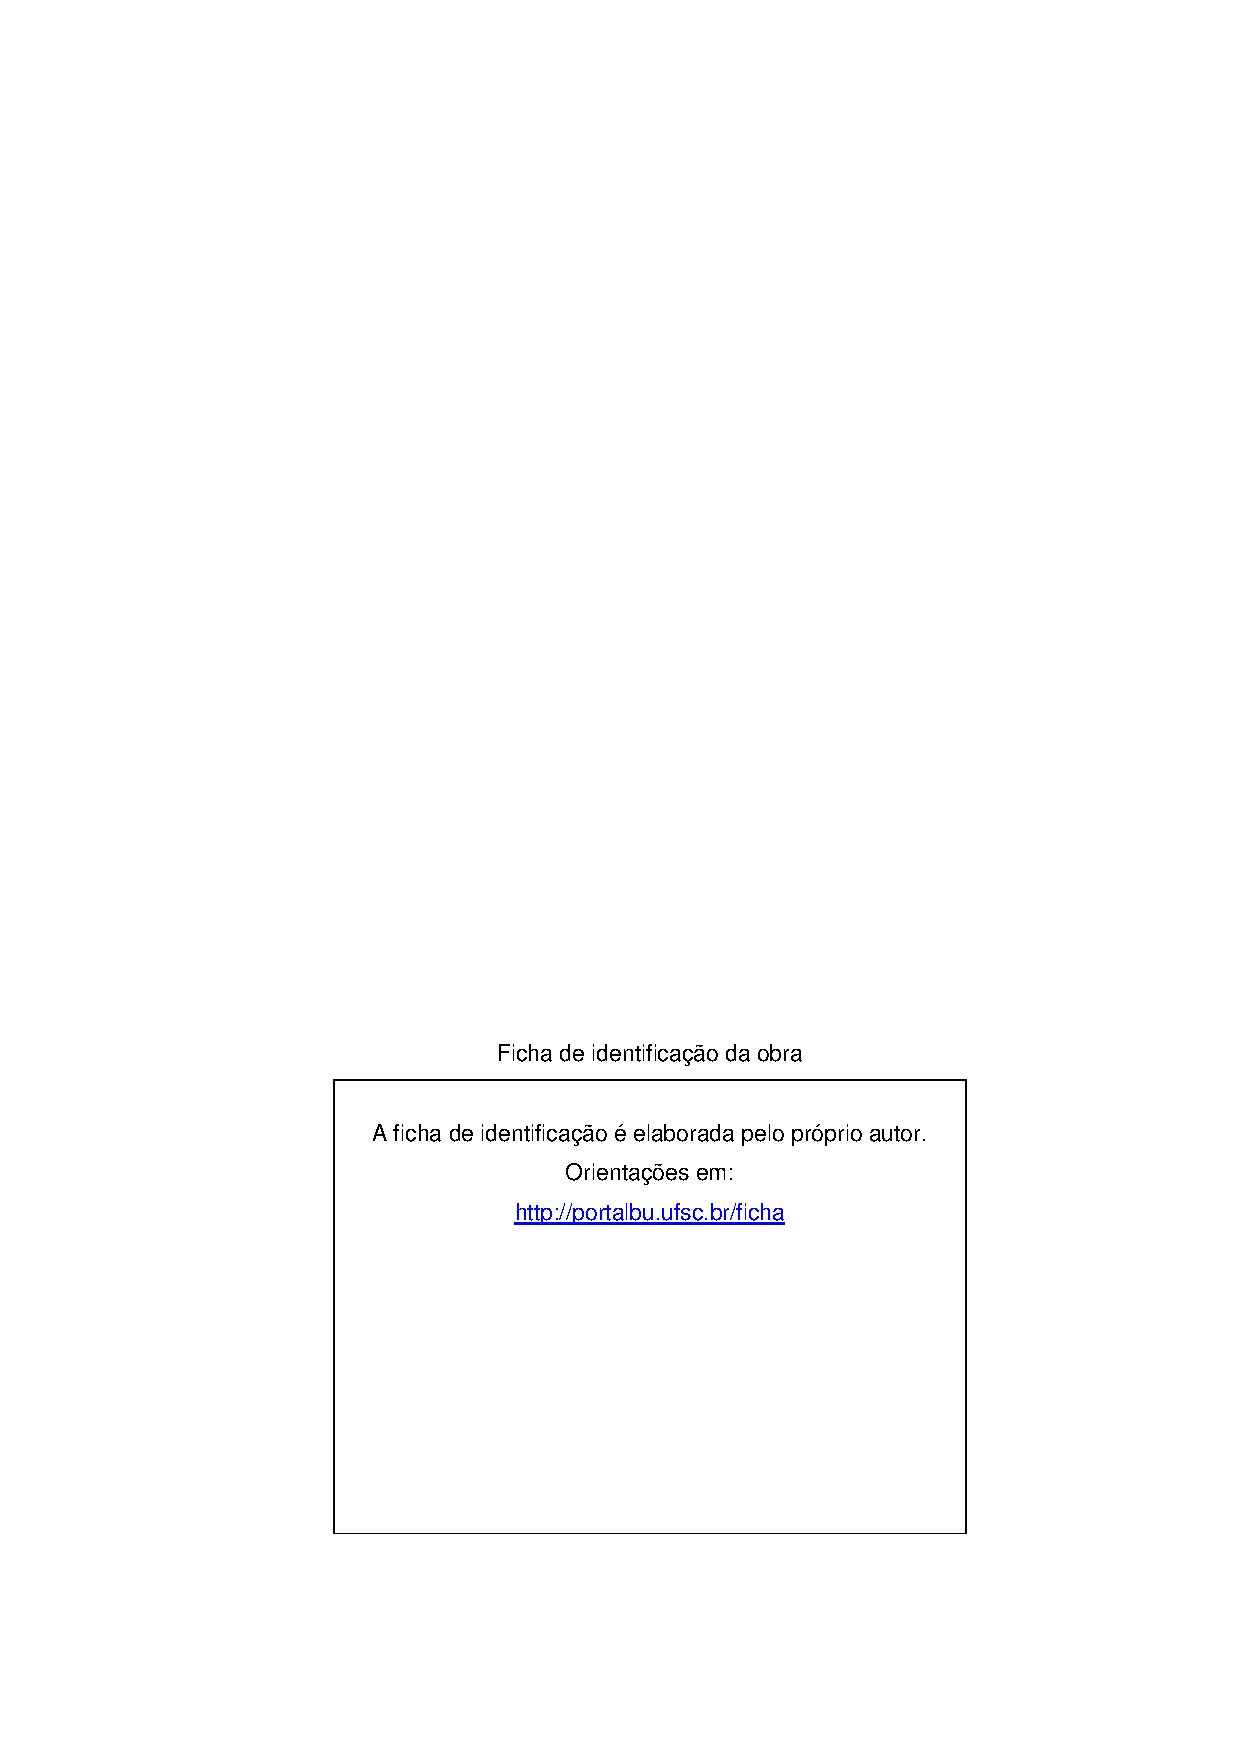
\includepdf{beforetext/Ficha_Catalografica.pdf}
\end{fichacatalografica}
% ---

% ---
% Inserir folha de aprovação
% ---
\begin{folhadeaprovacao}
	\OnehalfSpacing
	\centering
	\imprimirautor\\%
	\vspace*{10pt}		
	\textbf{\imprimirtitulo}%
	\ifnotempty{\imprimirsubtitulo}{:~\imprimirsubtitulo}\\%
	%		\vspace*{31.5pt}%3\baselineskip
	\vspace*{\baselineskip}
	
	Esta monografia foi julgada no contexto da disciplina DAS5511 (Projeto de Fim de Curso) e aprovada em sua forma final pelo \imprimircurso\\
	\vspace*{\baselineskip}
	Florianópolis, <dia(número)> de <mês> de <ano(número)>.\\
	
	%%%%%%%%%%%%%%%%%%%%%%%%%%%%%%%%%%%%%%%%%%%%%%%%%
	%IMPORTANTE: não é necessário assinaturas abaixo!
	%%%%%%%%%%%%%%%%%%%%%%%%%%%%%%%%%%%%%%%%%%%%%%%%%
	
	\vspace*{2\baselineskip}
	%\rule{0.4\textwidth}{0.4pt}\\
	Prof. Marcelo De Lellis Costa De Oliveira, Dr.\\
	Coordenador do Curso\\
	
	\vspace*{\baselineskip}
	\textbf{Banca Examinadora:} \\ \emph{[preencher somente após a defesa para a  Versão Final da BU]} \\
	
	
	\vspace*{2\baselineskip}
	%\rule{0.4\textwidth}{0.4pt}\\
	Prof(a). Carlos Barros Montez, Dr.\\
	Orientador(a) \\
	UFSC/CTC/EAS\\
	
	\vspace*{2\baselineskip}
	%\rule{0.4\textwidth}{0.4pt}\\
	Matheus Fischer, Eng.\\
	Supervisor(a) \\
	Fischertec Tecnologia\\
	
	\vspace*{2\baselineskip}
	%\rule{0.4\textwidth}{0.4pt}\\
	Prof(a). xxxx, Dr(a).\\
	Avaliador(a) \\
	Instituição xxxx\\
	
	\vspace*{2\baselineskip}
	%\rule{0.4\textwidth}{0.4pt}\\
	Prof. xxxx, Dr.\\
	Presidente da Banca \\
	UFSC/CTC/EAS
\end{folhadeaprovacao}
% ---

% ---
% Dedicatória
% ---
\begin{dedicatoria}
	\vspace*{\fill}
	\noindent
	\begin{adjustwidth*}{}{5.5cm} 
		\raggedleft       
		Este trabalho é dedicado aos meus colegas de classe e aos meus queridos pais.
	\end{adjustwidth*}
\end{dedicatoria}
% ---

% ---
% Agradecimentos
% ---
\begin{agradecimentos}
	Inserir os agradecimentos aos colaboradores da execução do trabalho. 
	
	Xxxxxxxxxxxxxxxxxxxxxxxxxxxxxxxxxxxxxxxxxxxxxxxxxxxxxxxxxxxxxxxxxxxxxx. 
\end{agradecimentos}
% ---

% ---
% Epígrafe
% ---
% \begin{epigrafe}
% 	\vspace*{\fill}
% 	\begin{flushright}
% 		\textit{``Texto da Epígrafe.\\
% 			Citação relativa ao tema do trabalho.\\
% 			É opcional. A epígrafe pode também aparecer\\
% 			na abertura de cada seção ou capítulo.\\
% 			Deve ser elaborada de acordo com a NBR 10520.''\\
% 			(SOBRENOME do autor da epígrafe, ano)}
% 	\end{flushright}
% \end{epigrafe}
% ---

% ---
% DECLARAÇÃO DE PUBLICIDADE
% ---

\begin{center}
	\textbf{DECLARAÇÃO DE PUBLICIDADE}
\end{center}

% Atenção: atualize o conteúdo de <texto>.

% <Nome da cidade>, <dia> de <mês> de <ano>.
Blumenau, 17 de janeiro de 2025.

\vspace{1cm}

Na condição de representante da <instituição de realização do PFC> na qual o presente trabalho foi realizado, declaro não haver ressalvas quanto ao aspecto de sigilo ou propriedade intelectual sobre as informações contidas neste documento, que impeçam a sua publicação por parte da Universidade Federal de Santa Catarina (UFSC) para acesso pelo público em geral, incluindo a sua disponibilização \emph{online} no Repositório Institucional da Biblioteca Universitária da UFSC. Além disso, declaro ciência de que o autor, na condição de estudante da UFSC, é obrigado a depositar este documento, por se tratar de um Trabalho de Conclusão de Curso, no referido Repositório Institucional, em atendimento à Resolução Normativa n° 126/2019/CUn.

Por estar de acordo com esses termos, subscrevo-me abaixo.

\vspace{15mm}

\begin{center}
	\rule{7cm}{0.7pt} \\
	Matheus Fischer, Eng. \\
	Fischertec Tecnologia
\end{center}

\cleardoublepage

% ---
% RESUMOS
% ---

% resumo em português
\setlength{\absparsep}{18pt} % ajusta o espaçamento dos parágrafos do resumo
\begin{resumo}
	\SingleSpacing
	\textbf{Instruções do padrão genérico de TCCs da BU:}
	No Resumo são ressaltados o objetivo da pesquisa, o método utilizado, as discussões e os resultados com destaque apenas para os pontos principais. O resumo deve ser significativo, composto de uma sequência de frases concisas, afirmativas, e não de uma enumeração de tópicos. Não deve conter citações. Deve usar o verbo na voz ativa e na terceira pessoa do singular. O texto do resumo deve ser digitado, em um único bloco, sem espaço de parágrafo. O espaçamento entre linhas é simples e o tamanho da fonte é 12. Abaixo do resumo, informar as palavras-chave (palavras ou expressões significativas retiradas do texto) ou, termos retirados de thesaurus da área. Deve conter de 150 a 500 palavras. O resumo é elaborado de acordo com a NBR 6028. 
	
	\textbf{Instruções da Coordenação de PFC:} O Resumo deve descrever de forma sucinta: o contexto/motivação/problema tratado no PFC; a solução proposta; a implementação/desenvolvimento; a metodologia e as principais técnicas e ferramentas utilizadas; os principais resultados obtidos e a importância/impactos de tais resultados para a empresa/clientes da empresa/instituto de pesquisa. Escrever todos esses pontos de forma bem resumida e direta, e sem entrar em detalhes técnicos. O tamanho do Resumo deve ocupar praticamente esta página inteira, e num \textbf{único} parágrafo. Além disso, Resumo + Palavras-Chave não podem ultrapassar esta página. 
		
	\textbf{Palavras-chave}: Palavra-chave 1. Palavra-chave 2. Palavra-chave 3. \emph{[essas palavras-chave devem obrigatoriamente ser utilizadas no Resumo]}
\end{resumo}

% resumo em inglês
\begin{resumo}[Abstract]
	\SingleSpacing
	\begin{otherlanguage*}{english}
		Resumo traduzido para outros idiomas, neste caso, inglês. Segue o formato do resumo feito na língua vernácula. As palavras-chave traduzidas, versão em língua estrangeira, são colocadas abaixo do texto precedidas pela expressão “Keywords”, separadas por ponto.
		
		\textbf{Keywords}: Keyword 1. Keyword 2. Keyword 3.
	\end{otherlanguage*}
\end{resumo}

%% resumo em francês 
%\begin{resumo}[Résumé]
% \begin{otherlanguage*}{french}
%    Il s'agit d'un résumé en français.
% 
%   \textbf{Mots-clés}: latex. abntex. publication de textes.
% \end{otherlanguage*}
%\end{resumo}
%
%% resumo em espanhol
%\begin{resumo}[Resumen]
% \begin{otherlanguage*}{spanish}
%   Este es el resumen en español.
%  
%   \textbf{Palabras clave}: latex. abntex. publicación de textos.
% \end{otherlanguage*}
%\end{resumo}
%% ---

{%hidelinks
	\hypersetup{hidelinks}
	% ---
	% inserir lista de ilustrações
	% ---
	\pdfbookmark[0]{\listfigurename}{lof}
	\listoffigures*
	\cleardoublepage
	% ---
	
	% ---
	% inserir lista de quadros
	% ---
	\pdfbookmark[0]{\listofquadrosname}{loq}
	\listofquadros*
	\cleardoublepage
	% ---
	
	% ---
	% inserir lista de tabelas
	% ---
	\pdfbookmark[0]{\listtablename}{lot}
	\listoftables*
	\cleardoublepage
	% ---
	
	% ---
	% inserir lista de abreviaturas e siglas (devem ser declarados no preambulo)
	% ---
	\imprimirlistadesiglas
	% ---
	
	% ---
	% inserir lista de símbolos (devem ser declarados no preambulo)
	% ---
	\imprimirlistadesimbolos
	% ---
	
	% ---
	% inserir o sumario
	% ---
	\pdfbookmark[0]{\contentsname}{toc}
	\tableofcontents*
	\cleardoublepage
	
}%hidelinks
% ---